\RequirePackage[l2tabu, orthodox]{nag}
\documentclass[a4paper]{article}
\usepackage[utf8]{inputenc}
\usepackage[T1]{fontenc}
\usepackage{lmodern}
\usepackage[pdftex, hidelinks,
            pdftitle={Flödesanimering i realtid med 3D-rotationsbrus},
            pdfauthor={Martin Estgren and and Rasmus Hedin and Alfred Rundquist and Erik S. V. Jansson},
            pdfsubject={Computer Graphics -- Animation -- Physical Simulation / Procedural Animation},
            pdfkeywords={curl-noise,animation,fluid simulation,navier-stokes,gpu,real-time}]{hyperref}

\usepackage{bm}
\usepackage{caption}
\usepackage{listings}
\usepackage{mathtools}
\usepackage[margin=0.8in]{geometry}
\usepackage[parfill]{parskip}
\usepackage[swedish]{babel}
\usepackage{algorithmic}
\usepackage{graphicx}
\usepackage{courier}
\usepackage{hyperref}
\usepackage{amsmath}
\usepackage{amssymb}
\usepackage{algorithm}
\usepackage{multicol}
\setlength{\columnsep}{0.5cm}
\usepackage[capitalize, noabbrev]{cleveref}
\usepackage[activate={true, nocompatibility}, final,
            tracking=true, kerning=true, spacing=true,
            factor=1100, stretch=10, shrink=10]{microtype}

\DeclareCaptionFormat{modifiedlst}{\rule{\textwidth}{0.85pt}\\[-2.9pt]#1#2#3}
\captionsetup[lstlisting]{format =  modifiedlst,
labelfont=bf,singlelinecheck=off,labelsep=space}
\lstset{basicstyle=\footnotesize\ttfamily,
        breakatwhitespace = false,
        breaklines = true,
        keepspaces = true,
        language = C++,
        showspaces = false,
        showstringspaces = false,
        frame = tb,
        numbers = left,
        numbersep = 5pt,
        xleftmargin = 16pt,
        framexleftmargin = 16pt,
        belowskip = \bigskipamount,
        aboveskip = \bigskipamount,
        escapeinside={<@}{@>}}

\date{\vspace{-0.5ex}} % Buys us some space.
\title{\vspace{-2.2cm}\textbf{Flödesanimering i realtid med 3D-rotationsbrus}\\
       \Large{\textit{--- en kort teknisk saga angående dess fasor och dess under ---}}\vspace{-0.25cm}}
\author{{\textbf{Martin Estgren}}\;\;\;\;\;\; {\href{mailto:mares480@student.liu.se}{\texttt{<mares480@student.liu.se>}}}\\
        {\textbf{Rasmus Hedin}}\;\;\;\;\;\;\;\; {\href{mailto:rashe877@student.liu.se}{\texttt{<rashe877@student.liu.se>}}}\\
        {\textbf{Alfred Rundquist}}\;\;\; {\href{mailto:alfru536@student.liu.se}{\texttt{<alfru536@student.liu.se>}}}\\
        {\textbf{Erik S. V. Jansson}}\; {\href{mailto:erija578@student.liu.se}{\texttt{<erija578@student.liu.se>}}}}

\begin{document}
    \maketitle
\begin{multicols}{2}

    \section{Introduktion}

    Ett viktigt område inom \emph{datorgrafik och visualisering} är förmågan att \emph{simulera}/\emph{animera} verklighetstrogna \emph{flödessystem} i \emph{realtid}. Dessa används i bl.a. spel och filmer för att enkelt skapa \emph{visuella effekter} som t.ex. \emph{rök- och vattenrörelser}; effekter som vanligtvis inte animeras ``för hand'', utan är mer lämpliga att generera i en dator. I detta projekt implementeras ett \emph{grundläggande flödessystem} för att \emph{animera ett partikelsystem} i 3D med hjälp av ett så kallat \emph{rotationsbrus} (``curl-noise''), först presenterad av \emph{Bridson et al.}~\cite{bridson2007curl} 2007.

    \textit{Rotationsbrus} används för att framställa verklighetstrogna \emph{partikelflöden} genom att procedurellt animera \emph{turbulenta flöden}. Detta görs genom att beräkna rotationen av ett vektorfält som genererats av \emph{procedurellt brus}. På så sätt skapas ett \emph{divergensfritt vektorfält}, som påverkar partiklarnas rörelsebanor utan att de ackumuleras på punkter i fältet. Metoden är ett billigare alternativ till \emph{Navier-Stokes}, som är fysiskt korrekt, men eftersom det i detta fall är främst de visuella egenskaperna som är intressanta, är rotationsbrus tillräckligt bra. Dessutom kan rotationsbrus beräknas i realtid, vilket gör den lämplig för integrering i t.ex. spel och informationsvisualisering.

	I originalrapporten presenteras beräkningar för både två och tre dimensioner men i detta projekt är endast det sistnämnda aktuellt. Dessutom är vissa beräkningar justerade för att bättre passa detta projekt.
	
    Målet med detta projekt var att skapa ett enkelt \emph{3D-partikelsystem} där partiklarnas rörelse bestäms av ett vektorfält genererat genom \emph{rotationsbrusmetoden} tillsammans med några enkla visuella effekter.

    Arbetsprocessen gick till stor del ut på parprogrammering, och versionshantering via \textit{Git}. För att realisera partikelsystemet användes \textit{OpenCL} för partikelberäkningar, \textit{OpenGL} för rendering, \textit{GLFW} för fönsterhantering, \textit{AntTweakbar} för ``run-time'' konfigurering, och \textit{GLEW} för att hantera \textit{OpenGL}-tillägg. Själva koden skrevs i C++ med \emph{Premake} som byggsystem, kernels skrevs i \textit{OpenCL} C variant, och shaders i \textit{GLSL}.

    \vspace{-0.5cm}
    \section{Teori och metodik}
    \vspace{-0.3cm}
    \subsection{Systemöversikt} \label{sec:system}

    Vid tidpunkten \(t_n\) befinner sig varje partikel vid sin egen position \(\vec{x}\), lagrad i en \emph{buffer}. Målet är att räkna ut partikelns nästa position \(\vec{x}'\) vid tidpunkten \(t_{n+1}\) (ett steg fram i simuleringen). Detta görs genom \(\vec{x}' = \vec{x} + \mathbf{\hat{V}}(\vec{x})\), där \(\mathbf{\hat{V}}(\vec{x})\) är \emph{fältriktningen}. Allt detta hanteras av \emph{partikelsystemet}, där dessutom \(\mathbf{\hat{V}}(\vec{x})\) skapas, och beskrivs under Rubrik~\ref{sec:partikelsystemet}. Detta görs parallellt på GPU:n för varje partikel under samma \(t_n\). Vilket gör att positionerna \(\vec{x}'\) kan återanvändas vid \emph{visualisering} i \emph{partikelrenderaren}, eftersom inget av systemen behöver lämna grafikprocessorns minnesrymd. Detta leder till god prestanda, och arbetstypen passar dessutom bra till sådana typer av processorer eftersom synkroniseringen är minimal. Se Figur~\ref{fig:system}.

    \begin{figure}[H]
    \center
    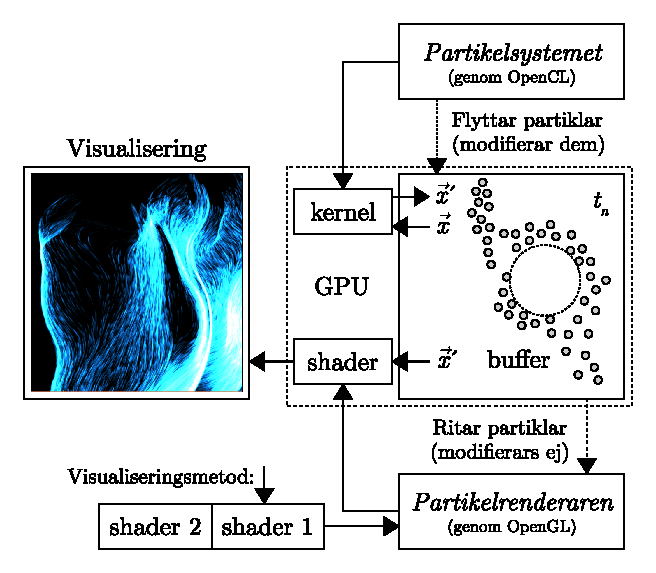
\includegraphics[width=0.5\textwidth]{share/System.eps}
    \caption{konceptuell översikt över de två subsystemen.}
    \label{fig:system}
    \end{figure}

    Detta görs genom att ladda upp en \emph{kernel} (beräkningskärna) som läser in \(\vec{x}\) och därefter skriver över denna med \(\vec{x}'\). Genom att läsa \(\vec{x}'\) från den delade buffern kan en \emph{shader} användas för att rita partiklarna, genom att tolka hela \(\vec{x}'\) som en \emph{vertex buffer}. Man kan enkelt ändra \emph{visualiseringsmetod} (hur man ritar \(\vec{x}'\)) genom att byta shader, vilket beskrivs under Rubrik~\ref{sec:partikelrenderaren}.

    \vspace{-0.35cm}
    \subsection{Partikelsystemet} \label{sec:partikelsystemet}

    Partikelsystemet bygger på att varje partikels nästkommande position beräknas parallellt av en \textit{OpenCL} kernel för varje frame. 

    I korthet kan man säga att tre olika vektorfält produceras och kombineras. De första två fälten representerar turbulensen och den allmänna riktningen som partiklarna ska följa. Dessa kombineras genom addition. Sedan modifieras resultatfältet så att partiklarna tar sig runt solida kroppar och slutligen appliceras en rotationsoperation (curl) vilket resulterar i ett divergensfritt vektorfält.

\begin{figure}[H]
\begin{minipage}[]{0.5\textwidth}
\center

\includegraphics[width=0.48\textwidth]{share/Noise_downscale.png}

\includegraphics[width=0.48\textwidth]{share/Background_downscale.png}

\vspace{0.1cm}


\includegraphics[width=0.48\textwidth]{share/Alpha_downscale.png}
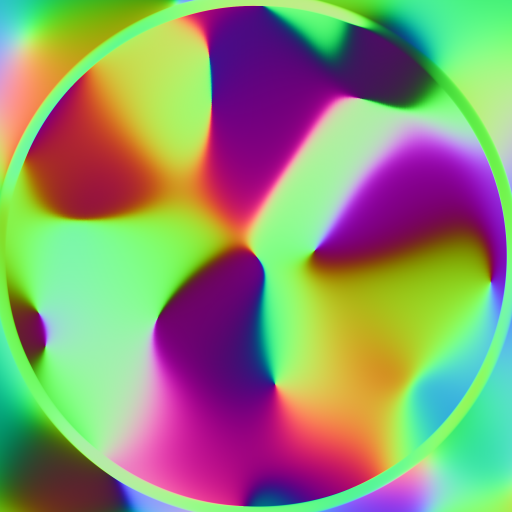
\includegraphics[width=0.48\textwidth]{share/Curl_downscale.png}
\end{minipage}
    \caption{$xy$-plan genomskärningar av  a) \emph{turbulensfältet} b) \emph{bakgrundsfältet} c) \emph{rampfunktionen} d) \emph{riktningsfältet}. (i den ordningen som visas: vänster$\rightarrow$höger, upp$\rightarrow$ner)}
\label{fig:curlnoise}
\end{figure}

\vspace{-0.3cm}
    \textbf{Turbulensfältet}

    Turbulensfältet beräknas genom att sampla en procedurell brusfunktion. Vi valde att använda \textit{Simplex noise}\footnote{\url{https://github.com/stegu/perlin-noise/blob/master/src/simplexnoise1234.c}} vilket förklaras i detalj av \emph{Stefan Gustavsson}~\cite{gustavson2005simplex}. Brusfunktionen samplas runt varje partikels position enligt följande funktion.
    \begin{equation}
   \vec{N}(\vec{x}) =
        \begin{pmatrix}
        n((\vec{x} + \vec{\epsilon}_x)/L)
        \\
        n((\vec{x} + \vec{\epsilon}_y)/L)
        \\ 
        n((\vec{x} + \vec{\epsilon}_z)/L)
        \end{pmatrix} * \gamma M_nL
    \end{equation}
    Där $\vec{\epsilon}$ representerar en förskjutning så att alla vektorkomponenter inte blir korrelerade med varandra. $n(\vec{x})$ är brusfunktionen som samplas för att producera turbulens i fältet. $\gamma$ representerar förhållande mellan brus och bakgrundsfält där $0$ är inget brus och därmed ingen turbulens medan $1$ är fullt brus utan något bakgrundsfält. $M_n$ är styrkan på bruset (fältriktningen är normerad så vi skalar upp det till vad vi vill ha). $L$ är längdskalan på bruset vilket i vårat fall är relativt stor (runt 20) då vi vill ha långa övergångar i bruset.

\textbf{Backgrundsfält}

Backgrundsfältet representerar den generella riktningen vi vill att partiklarna ska följa. Detta beskrivs inte något vidare i referensartikeln. Vi valde istället att anpassa en redan existerande implementation\footnote{\url{https://github.com/kbladin/Curl_Noise/blob/master/shaders/point_cloud_programs/update_velocities_curl_noise.frag}} av K. Bladin, vilket resulterar i ett bakgrundsfält som går i en uniform riktning efter att $\nabla \times$ operatorn har applicerats.
$     \vec{F}(\vec{x}) = (1.0-\gamma) *  \vec{D}(\vec{x}) * M_f $. $ \vec{D}(\vec{x})$ representerar fältriktningen i den angivna punkten och $M_f$ är magnituden vi vill ha. 

Fältriktningen är beräknad enligt följande formel $\vec{D}(\vec{x}) = \vec{x} \times \vec{p}$. Där $\vec{p}$ är fältriktningen vi vill att partiklarna ska följa.

\textbf{Solida kroppar}

Turbulensfältet adderas med backgrundsfältet ($\vec{\psi} = \vec{N}(\vec{x}) + \vec{F}(\vec{x})$) för att sedan justeras så att partiklarna beaktar solida sfärer utplacerade i vektorfältet. 

För att få alla partiklar att respektera de utplacerade sfärerna används rampfunktionen
\begin{equation}
ramp(r) = \left\{\begin{matrix}
1  && r > 1
\\
6r^4 - 15r^4 + 10r^3 && 0 \le r \le 1
\\ 
0  && r < 0
\end{matrix}\right.
\end{equation}
där $r$ är distansen $\vec{x}$ till närmaste sfär delat på distansen av sfären inflytande. 

Resultatet från rampfunktionen $\alpha = | ramp(d(\vec{x})/d_0) |$ där $d_0$  är en arbiträr skalfaktor. Slutligen beräknar vi fältet runt sfärerna genom 
\begin{equation}
\vec{\psi}_c(\vec{x}) = \alpha * \vec{\psi}(\vec{x}) + (1.0 - \alpha) * \hat{n} * \vec{\psi}(\vec{x}) \cdot \hat{n}
\end{equation}
där $\hat{n}$ är normalen från $\vec{x}$ till den närmsta sfären. Detta producerar en övergång från fältriktningen till en riktning tangentiell mot sfären.

\textbf{Curl}

Vi får fram $ \nabla \vec{\psi}$ genom en \textit{finit differensmetod} där vi samplar fältet väldigt nära punkten vi vill ha gradienten i och tar genomsnittet. Sist beräknas den slutgiltiga fältriktningen genom att applicera curl operatorn på vår framtagna gradient genom
\begin{equation}
\mathbf{\hat{V}}(\vec{x}) =
\nabla \times \begin{pmatrix}
\vec{vy}_z - \vec{vz}_y
\\ 
\vec{vz}_z - \vec{vx}_y
\\ 
\vec{vx}_z - \vec{vy}_y
\end{pmatrix} / 0.0002
\end{equation}
och normeras så att vi själva kan bestämma vad hastigheten för partiklarna ska vara. En genomskärning i $xy$-planet av dessa fält kan ses i Figur~\ref{fig:curlnoise}. 

\subsection{Partikelrenderaren} \label{sec:partikelrenderaren}

Då varje position \(\vec{x}\) finns tillgänglig i \emph{vertex shadern} (enligt Rubrik~\ref{sec:system}) kan vi ändra hur de ritas ut genom att modifiera senare \emph{shader ``pipeline'' steg}. Tre olika visualiseringsmetoder har implementerats, som beskrivs individuellt i kommande delar. Dessutom har vi valt att använda \emph{additiv färgblandning} när vi skriver till skärmbufferten, främst av estetiska skäl (områden med fler partiklar ger ett intryck att det är ``ljusare''), men dessutom av rent praktiska skäl (som kommer förklaras i kommande delar). Bilder över dessa visualiseringsmetoder finns i Rubrik~\ref{sec:results}.

\textbf{Punktvisualiseringen}

Den enklaste typen av visualisering är att bara skapa en ``punkt'' där partikeln bör ligga. Här behöver vi endast en \emph{vertex shader} och en \emph{fragment shader}. Då användaren ska kunna observera scenen från flera håll, måste positionerna \(\vec{x}\) omvandlas till det korrekta koordinatsystemet, \(\mathbf{MVP}\vec{x}\) i \emph{vertex shadern}. Därefter ger vi punkten en enkel färg genom att sätta resultatet från \emph{fragment shadern} till \(\begin{bmatrix}|x| & |y| & |z| & 1.0\end{bmatrix}\). Det vill säga, färgen av partikeln ges av dess position \(\vec{x}\).

\textbf{Billboardsvisualiseringen}

Visuella effekter så som eld och rök kan enkelt representeras med hjälp av s.k. \emph{``billboards''} (alt. \emph{``impostors''}), som är ett texturerat plan som alltid är riktad mot åskådaren (vilket ger intrycket att den är 2-D). Detta görs enligt \emph{Ingemar Ragnemalm}~\cite{ragnemalm2008polygons} enligt: \[\mathbf{M} = \begin{bmatrix} 1 & 0 & 0 & x \\
                                    0 & 1 & 0 & y \\
                                    0 & 0 & 1 & z \\
                                    0 & 0 & 0 & 1 \end{bmatrix}, \;
          \vec{x} = \begin{bmatrix}x & y & z\end{bmatrix}.\]

Hur skapas detta plan, givet en punkt \(\vec{x}\)? Då vi har valt att göra allt detta i våra shaders, måste vi \emph{skapa ny geometri} under körtid. Man gör detta med hjälp av en s.k. \emph{geometry shader}, ett steg som ligger mellan en \emph{vertex shader} och en \emph{fragment shader}.

\vspace{-0.3cm}
\begin{figure}[H]
\center
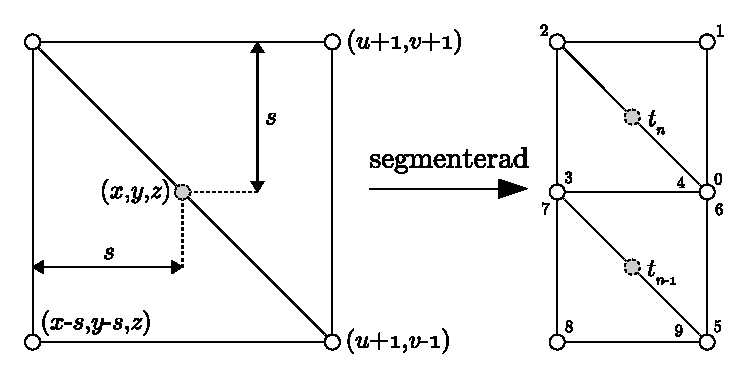
\includegraphics[width=0.5\textwidth]{share/Billboards.eps}
\caption{(a) en billboard (b) segmenterade billboards.}
\label{fig:bill}
\end{figure}
\vspace{-0.3cm}

Som figur~\ref{fig:bill}~(a) visar, skapar geometry shadern för varje punkt \(\vec{x}\) (representerad som en grå cirkel i figuren), 4 nya hörn centrerade runt \(\vec{x}\) (de vita cirklarna) genom \texttt{EmitVertex}. Dessa flyttats med \(s\) enheter åt respektive håll; en parameter som bestämmer hur stor planet ska vara. Man genererar primitiver (trianglar i detta fall) genom att anropa \texttt{EndPrimitive}. Sist sätter vi \((u, v)\)-koordinaterna för de hörn vi skapat, och använder dessa i \emph{fragment shadern} för att rita ut en 2-D textur som har ``häftats'' till/på vårat plan.

\textbf{Vektorfältvisualiseringen}

För att enklare kunna visualisera riktningsfältet har vi implementerat \emph{``glyphs''}, som bl.a. beskrivs i \emph{McQuinn et al.}~\cite{mcquinn2013glyphsea}. Tekniken går ut på att ``dra ut'' en billboard så att den följer fältets riktning. Vi har gjort en förenklad variant, där de \(k\) senaste \(\vec{x}\)-värdena (vid tidsteg \(t_{n-1}, ..., t_{n-k}\)) lagras i en \emph{cirkulär buffer} \(\mathcal{C}\). Dessa används för att skapa en \emph{segmenterad billboard}, där de olika segmenten skapas mellan två punkter \(\vec{x}_{i-1}\),~\(\vec{x}_i\), där \(\vec{x}_{i-1}\),~\(\vec{x}_i\)~\(\in \mathcal{C}\). För varje segment skapas två hörn vid sidan av \(\vec{x}_i\) och två hörn vid sidan av \(\vec{x}_{i-1}\) enligt figur~\ref{fig:bill}~(b), som sedan används för att generera primitiver för varje segment (som kopplas samman).

\subsection{De övriga teknikaliteterna}

\textbf{Grafiska gränssnittet}

\textit{AntTweakBar} användes för att på ett smidigt sätt få ett grafisk gränssnitt där man kan ändra parametrar under körtid. När allt för en frame har renderats, så ritas gränssnittet ut ovanpå allt med \texttt{TwDraw}. Som man kan se i figur~\ref{fig:atb} har vi lite olika parametrar som kan ändras för att få olika visuella effekter. Exempelvis kan man ändra riktningen på bakgrundsfältet, andel brus, och välja hur partiklarna ska visualiseras.

\begin{figure}[H]
\center
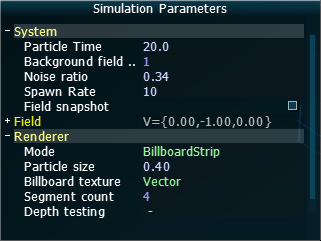
\includegraphics[width=0.48\textwidth]{share/atb.png}
\caption{Grafiska gränssnittet använder \textit{AntTweakBar}}
\label{fig:atb}
\end{figure}

\textbf{Kamerasvep}

För att enkelt röra sig mellan olika perspektiv i scenen så har vi definierat ``områden av intresse'' där kameran bör vara (och i vilken riktning).  För att få mjuka kameraövergångar interpolerades kamerans position med en \emph{ease in/out}-funktion, med tiden som parameter.

\section{Resultat \& diskussion} \label{sec:results}

En teknisk ``demo'' har byggts med metoderna som har beskrivits, och ett exempel av resultaten kan ses vid Figur~\ref{fig:verysexy}. Våran implementation klarar av att trivialt animera och rendera 10 000 aktiva partiklar i realtid (60 FPS) med en NVIDIA GTX 980ti.

All kod\footnote{\url{http://github.com/CaffeineViking/cnpf}} är open-source och delas under en permissiv licens, som kan byggas till Windows och Linux.

\begin{figure}[H]
\center
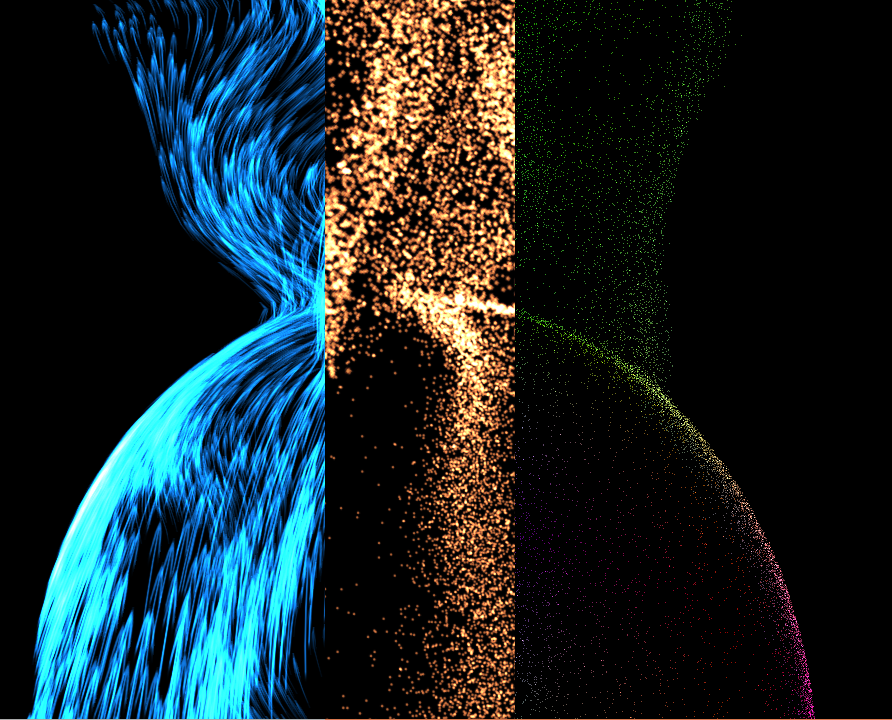
\includegraphics[width=0.48\textwidth]{share/merged_shaders.png}
    \caption{visualisering av \emph{partikelsystemet} med tre olika metoder: \emph{vektorfält-}, \emph{billboard-}, och \emph{punktvisualisering} som drivs av \emph{partikelrenderaren}. Scenariot innehåller en solid sfärisk kropp och med en längdskala på \(L\approx20\).}
\label{fig:verysexy}
\end{figure}

        \subsection{Problem samt lösningar}

            \textbf{``Svarta hål'' av ej divergensfrihet}

            Tidigt i projektet hade vi problemet att partiklar konvergerade mot vissa punkter. Något som ej borde inträffa, då curl-noise skall vara ett divergensfritt vektorfält. Det visade sig (med examinatorns hjälp) att linjära interpoleringen som gjordes av riktningsfältet i GPU:n förstörde den egenskapen. Evaluering av riktningsfältet på GPU:n kontinuerligt löste de problemen.

            \textbf{Interpoleringsfel av CPU Simplex}

            Något liknande inträffade senare i projektet, där våra partiklar tenderade att röra sig mot en viss riktning. Till slut visade det sig att detta inträffade för att vi interpolerade simplexbruset och samplade alla komponenter på samma position. Genom att introducera $\vec{\epsilon}$ och flytta över samplingen till GPU:n så att vi inte behövde lagra det i en 3D textur löste sig problemet.

            \textbf{Konstigheter i ``geometry shader''}
            
            För att få segmenterade billboards att fungera behövde partiklarnas gamla positioner samplas och skickas till en ``geometry shader''. En buffer med plats för alla samplade gamla positioner användes av OpenCL. Att direkt föra över delar av denna buffer till en buffer i OpenGL fungerade inte och gav bara positioner i origo. Ett nytt försök gjordes med en separat buffer (den \(\mathcal{C}\) i rapporten) för varje tidpunkt. Alltså, för varje tidpunkt finns en buffer med alla partiklars gamla positioner för den tidpunkten. Detta var en lösning till problemet, och vi hade nu tillgång till alla tidigare positioner som behövdes för att skapa segmenterade billboards.
            
            Ett annat problem som dök upp var att det saknades delar av våra billboards när de skulle ritas ut. Orsaken till problemet var att för varje segment skapades bara 4 hörn som sedan skulle bindas ihop till en quad vilket inte gav rätt resultat. Lösningen var att skapa varje quad med två polygoner manuellt (Se figur~\ref{fig:bill}). 
            % ...

        \subsection{Framtida förbättringar}

            \textbf{Segmentering med ``B-splines''}

            Eftersom vi har en minnesbegränsning på \(\mathcal{C}\) kan vi endast segmentera billboards till en viss nivå tills det börjar bli ``dyrt''. Här kan vi använda en \emph{B-spline} för att interpolera mjukt t.ex. \(\sum \vec{x}_i N^3_i(t)\), mellan den ändliga mängden kontrollpunkter och få ``fler'' \(\vec{x}_i\).

            \textbf{Filformat för ``egna'' scenarion}

            Att kunna modifiera upplägget med en egen fil (t.ex. i JSON eller XML) skulle ha gjort våra demon mer flexibla för att skapa scenarion snabbare. Exempelvis att kunna bestämma shaders, flera solida kroppar och möjligtvis omgivning (ladda in 3-D modeller).

            \textbf{Konkreta scenarion av shaders}

            Några mer ``praktiskt relevanta'' shaders och scenarion skulle ha varit intressanta att ha i demonstrationen. Exempelvis, att ha en gryta över en brasa som dessutom skapar lite rök. Det skulle innehålla all teknik som finns i detta projekt, dock krävs mer kod.

        \subsection{Projektreflektioner}

            Över lag är vi mycket nöjda med resultatet. När vi gick in i detta projekt hade vi inte mer än en väldigt otydlig bild av vad som skulle göras. Genom projektets gång har vi progressivt utvecklat vår vision om vad vi ville se i slutet och hur det skulle implementeras.

    \nocite{*} % Include all.
    \bibliographystyle{abbrv}
    \bibliography{cnpf}
\end{multicols}
\end{document}
